% Vektorgrafiken der Ganzzahl-Lesefassung. Die Edition lädt TikZ.
\definecolor{integersblue}{RGB}{34,92,133}
\definecolor{integersgreen}{RGB}{49,112,81}
\definecolor{integersgray}{RGB}{104,111,119}

\newcommand{\IntegersPairGrid}{%
  \par\medskip\noindent
  \begin{minipage}{\linewidth}
  \centering
  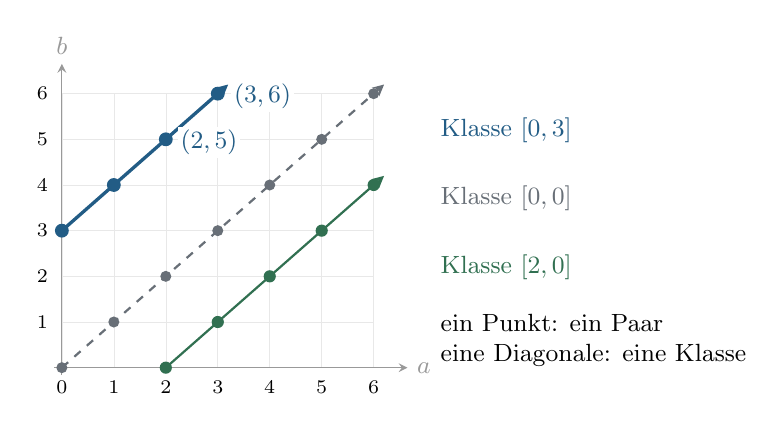
\begin{tikzpicture}[x=.66cm,y=.58cm,font=\small,>=stealth]
    \draw[step=1,gray!18,very thin] (0,0) grid (6,6);
    \draw[->,gray!80] (-.15,0)--(6.65,0) node[right] {\(a\)};
    \draw[->,gray!80] (0,-.15)--(0,6.65) node[above] {\(b\)};
    \foreach \k in {0,...,6} {
      \node[below,font=\scriptsize] at (\k,-.07) {\(\k\)};
    }
    \foreach \k in {1,...,6} {
      \node[left,font=\scriptsize] at (-.08,\k) {\(\k\)};
    }
    \draw[->,integersgray,dashed,thick] (0,0)--(6.2,6.2);
    \draw[->,integersgreen,thick] (2,0)--(6.2,4.2);
    \draw[->,integersblue,very thick] (0,3)--(3.2,6.2);
    \foreach \k in {0,...,6} {
      \fill[integersgray] (\k,\k) circle (2pt);
    }
    \foreach \a/\b in {2/0,3/1,4/2,5/3,6/4} {
      \fill[integersgreen] (\a,\b) circle (2.2pt);
    }
    \foreach \a/\b in {0/3,1/4,2/5,3/6} {
      \fill[integersblue] (\a,\b) circle (2.5pt);
    }
    \node[anchor=west,text=integersblue,fill=white,inner sep=1pt]
      at (2.22,4.93) {\((2,5)\)};
    \node[anchor=west,text=integersblue,fill=white,inner sep=1pt]
      at (3.25,5.94) {\((3,6)\)};
    \node[anchor=west,text=integersblue] at (7.1,5.2)
      {Klasse \([0,3]\)};
    \node[anchor=west,text=integersgray] at (7.1,3.7)
      {Klasse \([0,0]\)};
    \node[anchor=west,text=integersgreen] at (7.1,2.2)
      {Klasse \([2,0]\)};
    \node[anchor=west,align=left] at (7.1,.6)
      {ein Punkt: ein Paar\\eine Diagonale: eine Klasse};
  \end{tikzpicture}
  \par\smallskip\small\raggedright
  Drei Klassen im Ausschnitt des natürlichen Paargitters.
  Die Gitterpunkte derselben Diagonalen erfüllen die
  Kreuzsummengleichung. Jede Diagonale setzt sich nach rechts oben
  fort; die ganze Klasse enthält auch die nicht eingezeichneten Paare.
  \end{minipage}\par\medskip
}

\newcommand{\IntegersTwoRays}{%
  \par\medskip\noindent
  \begin{minipage}{\linewidth}
  \centering
  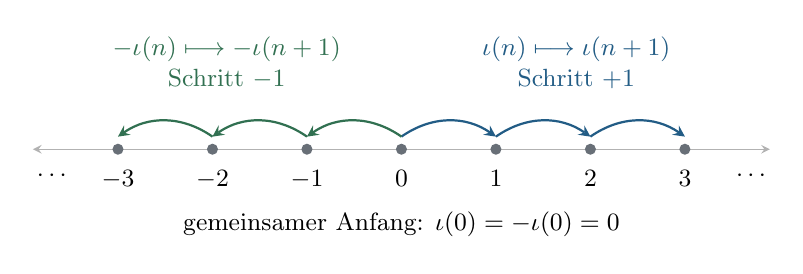
\begin{tikzpicture}[x=1.2cm,y=1cm,font=\small,>=stealth]
    \draw[<->,gray!60] (-3.9,0)--(3.9,0);
    \foreach \k in {-3,...,3} {
      \fill[integersgray] (\k,0) circle (2pt);
      \node[below=4pt] at (\k,0) {\(\k\)};
    }
    \node[below=4pt] at (-3.7,0) {\(\cdots\)};
    \node[below=4pt] at (3.7,0) {\(\cdots\)};
    \foreach \k in {0,1,2} {
      \draw[->,thick,integersblue]
        (\k,.16) to[bend left=35] (\k+1,.16);
      \draw[->,thick,integersgreen]
        (-\k,.16) to[bend right=35] (-\k-1,.16);
    }
    \node[text=integersgreen,align=center] at (-1.85,1.1)
      {\(-\iota(n)\longmapsto-\iota(n+1)\)\\Schritt \(-1\)};
    \node[text=integersblue,align=center] at (1.85,1.1)
      {\(\iota(n)\longmapsto\iota(n+1)\)\\Schritt \(+1\)};
    \node[below=19pt,align=center] at (0,0)
      {gemeinsamer Anfang: \(\iota(0)=-\iota(0)=0\)};
  \end{tikzpicture}
  \par\smallskip\small\raggedright
  Beide Induktionen verwenden einen natürlichen Zählparameter
  \(n=0,1,2,\ldots\). Auf dem positiven Strahl wird dabei eins
  addiert, auf dem negativen eins subtrahiert. Die Normalform zeigt,
  dass beide Strahlen zusammen alle ganzen Zahlen erfassen.
  \end{minipage}\par\medskip
}
